\section{Our work}
The x-vector architecture has significantly outperformed the traditional statistical approaches and is very popular model to the date, although it is not state of the art anymore. Besides different newer architectures, the original x-vector model performance was further improved using different training methods and loss functions. In~\cite{x_vectors_triplet}, they used multi-task training to train the model and had visible improvements in performance metrics compared with original training method. They enhanced cross-entropy loss from softmax activation with direct optimization on L2 distances between embeddings from hidden layer using triplet margin loss. They also used small neural network to extract more complex distance metric.

\medskip
Goal of our work was to test different loss functions separately to see their potential to train x-vector architecture and infere their contribution in multi-task losses. As a backend scoring metric, we used cosine similarity as a very strong and popular metric. Another popular backend in recent years is PLDA~\footnote{https://towardsdatascience.com/probabilistic-linear-discriminant-analysis-plda-explained-253b5effb96}, but lately it lost its popularity due to the increasing capabilities of DNN models. The main reason why we didn't choose PLDA is that it is a classifier and has hyperparameters, which might shadow the actual DNN model performance. 

\subsection*{Implementation and dataset}

We build the model using pytorch library in order to get more flexibility, despite the fact the model used in production is already implemented in popular C++ Kaldi library. We decided to use the smaller version of the new VoxCeleb~\cite{VoxCeleb} dataset, which consists of 148 642 utterances from 1211 speakers in the training set, and 4874 utterances from 40 speakers in the test set, all from YouTube videos. We preprocessed each utterance before the training step. We used single channel audio with 16kHz sampling rate as a raw input. Preemphasis with coeficient 0.97 has been then applied and the audio has been divided into overlapping frames each of length of 25 milliseconds and with step of 15 milliseconds between adjacent frames. For each frame, the STFT~\footnote{Short Time Fourier Transform} has been computed and finally the 128-dimensional spectrogram has been extracted using Mel frequency filter banks. In traditional approaches, the high correlation in this spectrogram used to be undesirable, but in DNN approaches more dimensionality has been shown to yield better results~\cite{CNN_2016}. However, we used a decorrelated spectrogram -- the MFCC~\footnote{https://haythamfayek.com/2016/04/21/speech-processing-for-machine-learning.html}, because in the original x-vector paper they used those. Initially we wanted to test both, but soon we realized that our hardware might not let us to do so, and we decided to use a 24-dimensional MFCC features only as a input to the model. For all these audio processing tasks, we used python framework librosa. We've implemented and used 3 training methods, each defined by different loss function.

\subsection*{Softmax with cross-entropy}

We trained the first model using original training method, i.e. closed set classification trying to classify respective utterances to each speaker in the training dataset. The multiclass cross-entropy loss function on softmax activation of the last layer~(eq. \ref{eq:softmax}) has been optimized.

\begin{equation} \label{eq:softmax}
\mathcal{L}_{softmax} = \frac{1}{N} \sum - \textnormal{log} \left( 
\frac{e^{\,\boldsymbol{x} \cdot \boldsymbol{W}_i^T + \boldsymbol{b}_i}}
{\sum_{j} e^{\,\boldsymbol{x} \cdot \boldsymbol{W}_j^T + \boldsymbol{b}_j}} 
\right)
\end{equation}

\pagebreak
\noindent
We trained the network using Adam optimizer with default parameters while it was seemingly converging and then tuned it using SGD with momentum $ 0.9 $ and small $ \eta = 1e^{-4} $. The training has been done on variable length utterances with minibatch size of 64. We used a cross-validation set created from the training set to determine the convergence of the optimizer.

\subsection*{Triplet margin loss -- direct optimization}

The second approach we've tested is direct optimization using standard triplet margin loss (eq. \ref{eq:triplet}) with L2 distance, where $ \boldsymbol{A} $, $ \boldsymbol{P} $ and $ \boldsymbol{N} $ are embedding vectors for anchor, positive (from the same speaker), and negative (from a different speaker) utterances respectively. The triplet loss is minimized, when for every speaker the intra-class distances are all smaller than inter-class distances by a margin of $ \alpha $.

\begin{equation} \label{eq:triplet}
\mathcal{L}_{triplet} = \frac{1}{N} \sum \textnormal{max}
\left( 
\norm{\boldsymbol{A} - \boldsymbol{P}}^2 - 
\norm{\boldsymbol{A} - \boldsymbol{N}}^2 
+ \alpha, 0 \right)
\end{equation}

\noindent
The one benefit of this approach over classification is obvious -- it does not require exact class annotations as closed set classification does. But from the performance perspective, it is not so obvious. One might argue that direct training should lead to better results, but softmax with more than thousand classes is forced to learn very discriminative representation and the optimization takes all those classes into account in every learning step. It is known that whereas triplet learning for embedding extraction is capable to outperform other approaches, it is crucial to employ good sampling technique and use hard-negative~mining~\cite{YuanYZ16}.

\medskip
In our work, we've implemented naive sampling where all triplets are sampled randomly with uniform probability during the whole training. Another important thing about triplet margin loss is its hyperparameter $ \alpha $. We used the value of 0.8 as recommended in~\cite{x_vectors_triplet}. The ReLU activation from the embedding layer has been removed and also the output embeddings were normalized in order to prevent network from degrading into extremely increasing or decreasing the embedding magnitude without changing its orientation (and cosine similarity backend score). We trained the model in a similar manner as the previous one.

\subsection*{Angular Softmax with cross-entropy}

The third and the last loss function we've tested is so called Angular~Softmax~loss~\cite{A_softmax_original} or A-softmax. It is a relatively recent approach to the problem of classic softmax activation used for embedding extraction. In classification using softmax, there is no direct way of maximizing the inter-class variability and minimizing the intra-class variability, which is desired property for a good embedding model. The final cross-entropy loss is not forced to keep any margins, it only cares about classifying the samples into the classes correctly in a discreet sense. The angular softmax can be viewed as an enhanced softmax idea based on the geometric definition of the dot product, which implies the equivalence~(eq. \ref{eq:cosine_rule}), where $ \theta_i $ is the angle between the class weights $ \boldsymbol{W}_i $ (column of the linear layer matrix for row vector convention) and the input vector $ \boldsymbol{x} $.

\begin{equation} \label{eq:cosine_rule}
\frac{e^{\,\boldsymbol{x} \cdot \boldsymbol{W}_i^T + \boldsymbol{b}_i}}
{\sum_{j} e^{\,\boldsymbol{x} \cdot \boldsymbol{W}_j^T + \boldsymbol{b}_j}} =
\frac{e^{\norm{\boldsymbol{x}} \cdot \norm{\boldsymbol{W}_i} \textnormal{cos}(\theta_i)  + \boldsymbol{b}_i}}
{\sum_{j} e^{\norm{\boldsymbol{x}} \norm{\boldsymbol{W}_j} \textnormal{cos}(\theta_j)  + \boldsymbol{b}_j}}
\end{equation}

\medskip
\noindent
The main idea is to multiply the angle $ \theta_i $, i.e. angle between $ x $ and weights of the ground-truth class by some value $ m $. Because the cosine function is monotonically decreasing in the interval $ \langle 0, \pi \rangle $, the relation $ j \neq i : \textnormal{cos}(\theta_i) > m \cdot \textnormal{cos}(\theta_i) > \textnormal{cos}(\theta_j) $ holds true in this interval. In~\cite{A_softmax_original} it is also shown that this new restriction creates angular margin between weight vectors of different classes. This margin forces the model to learn more discriminative features, because it has to minimize the angles within classes and maximize the angles between classes. Recently, there have been more losses with such margins, e.g. Additive Angular Margin Loss \cite{arc_face} where $ m $ is incorporated using addition instead of multiplication, but in~\cite{A_softmax} they used the hyper-spherical loss based on multiplication for a speaker verification task, so we did the same.

\medskip
We've implemented a linear layer without 	bias and with weights L2 normalization (as recommended). We used the value $ m = 3 $, which has been suggested in~\cite{A_softmax} to be the optimal. They also recommended the integral value of $ m $, so the multi-angle formula could be used to simplify backward gradient computations. In our case of $ m = 3 $, it can be simplified using the formula (eq. \ref{eq:multi_angle_3}). Finally, to remove the restriction of $ \theta_i $ being in interval $ \langle 0, \frac{\pi}{m} \rangle $, the new function has been introduced to replace the cosine (eq. \ref{eq:new_function}).

\begin{equation} \label{eq:multi_angle_3}
\textnormal{cos}(3\theta) = 
4\textnormal{cos}(\theta)^3 - 3\textnormal{cos}(\theta) = 
4 \left( \frac{\boldsymbol{x} \cdot \boldsymbol{W}}{\norm{\boldsymbol{x}}} \right) ^3 - 
3 \left( \frac{\boldsymbol{x} \cdot \boldsymbol{W}}{\norm{\boldsymbol{x}}} \right)
\end{equation}
\begin{equation} \label{eq:new_function}
\phi \left( \theta_i \right) = 
(-1)^k \textnormal{cos} \left( m \theta_i \right) - 2k
\end{equation}

\medskip
\noindent
Now the final A-softmax loss function can be formulated by an expression (eq. \ref{eq:A_softmax}).

\begin{equation} \label{eq:A_softmax}
\mathcal{L}_{A-softmax} = \frac{1}{N} \sum - \textnormal{log} \left( 
\frac{e^{\norm{\boldsymbol{x}} \phi(\theta_i)}}
{\sum_{j \neq i} e^{\,\boldsymbol{x} \cdot \boldsymbol{W}_j^T}}
\right)
\end{equation}

\medskip
\noindent
The training process was not trivial in this case. We found out, that such restrictive loss metric is very prone to divergence at the beginning of the optimization (as also mentioned in~\cite{arc_face}). However, in~\cite{A_softmax} they didn't mention this problem, probably because they were able to use very large batches (1000) as they were not training the network on variable length utterances but only on chunks, and they also had better hardware than we did. To tackle this problem, we trained our network with help of softmax activation combined with A-softmax (eq. \ref{eq:combined_loss}), where we initially started with $ \alpha = 0.2 $ and $ \beta = 0.8 $.

\begin{equation} \label{eq:combined_loss}
\mathcal{L} = \alpha \cdot \mathcal{L}_{A-softmax} + \beta \cdot \mathcal{L}_{softmax}
\end{equation}

\medskip
\noindent
Then we slowly moved the coeficients towards $ \alpha = \beta = 0.5 $ (1 epoch for every step of $ 0.1 $) and then we finally removed the helper softmax loss and trained only using A-softmax until the convergence. We used the same strategy as before, i.e. Adam to converge fast somewhere and then SGD with reasonably small $ \eta $ to settle down in the local minima more precisely.

\section{Results}

The trained models were tested using mentioned cosine similarity metric on the testing dataset. The embeddings were computed for each utterance and then all embeddings were paired into a $ 4874 \times 4874 $ score matrix. Finally, the DET~\footnote{Detection Error Tradeoff} curves were plotted and the scalar metric EER~\footnote{Equal Error Rate} has been computed. This metric is a standard way to describe the performance of the binary hypothesis tests. It is very popular in evaluation of biometric systems such as speaker verification model. The metric represents the threshold for which the FPR~\footnote{False Positive Ratio} and FNR~\footnote{False Positive Ratio} values are equal. The threshold is not meant in an absolute way, but normalized into interval $ \langle 0, 1 \rangle $ in order to be invariant. Our results are summarized in the table~\ref{tab:eer}.

\begin{table}[h]
    \centering
    \begin{tabular}{|l|r|}
    \hline
        \textbf{Training Loss} & \textbf{EER} \\ \hline
        softmax & 12.34 \% \\ \hline
        softmax with ReLU & 10.66 \% \\ \hline
        A-softmax & 8.04 \% \\ \hline
        triplet margin L2 & 16.46 \% \\ \hline
    \end{tabular}
    \caption{Equal Error Rate values for different embedding models}
    \label{tab:eer}
\end{table}


\medskip
\noindent
As can be seen, the triplet margin loss with naive sampling performed the worst given the scoring backend. It might definitely improve the performance of the softmax in multi-task training, but on its own it would require avanced sampling technique and also experimentation with the margin $ \alpha $. Also, the L2 distance on normalized vectors is still slightly different than the cosine distance used for scoring, so maybe exploiting our backend decision and using cosine distance in triplet loss would yield better results. However, to test this hypothesis is out of the scope of our work. On the other hand, the Angular Softmax loss function has gained the best performance. The power of the central softmax based loss with large number of classes combined with additional angular margin led to superior results.

\medskip
There is an open debate about whether to use only linearly activated layer or with some non-linear activation on top of it as an embedding. In triplet margin loss the answer is clear, but in classification based embeddings we tried both variants and found interesting results. While the A-softmax with ReLU activation kept performed much worse, even worse than softmax, the plain softmax performed significantly better with ReLU than with ReLU removed. We suppose that the reason for this is that the ReLU discards information contained in the negative values. Therefore it is not propagated directly to the final minimized loss, so it can be expected that using the negative part would more likely confuse the results rather than improve them. But this explanation ostensibly doesn't apply for the A-softmax function. Interesting future work would be to test whether some other activations that keep also the negative part (e.g. tanh) would lead to even better results than classical ReLU, which is extensively used due to its great gradient properties, but those are not so significant after batch normalization anyway.

\medskip
Finally, we've also visualized the results in the form of DET~curves~(fig. \ref{fig:det}) and scatter~plots~\ref{fig:tsne} of the test utterances embeddings in 512 dimensional space reduced into 2 dimensions mantaining the L2 distances using t-SNE~\footnote{https://towardsdatascience.com/an-introduction-to-t-sne-with-python-example-5a3a293108d1} algorithm.

\begin{figure}[h]
\begin{center}
	\begin{subfigure}[t]{7.5cm}
		\resizebox{7.5cm}{!}{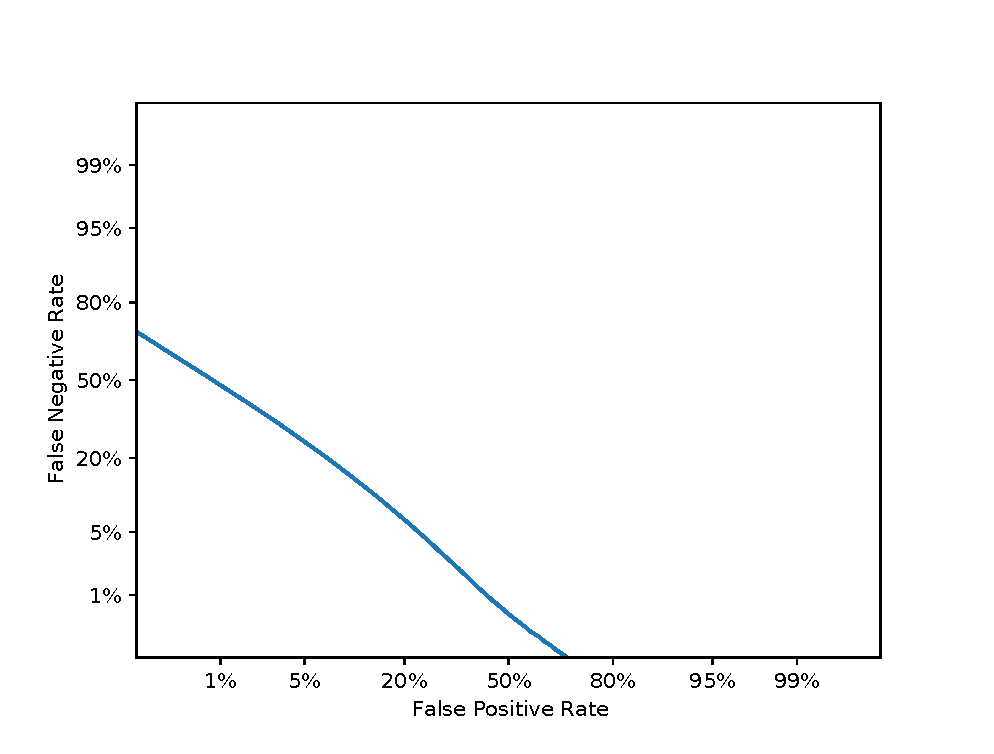
\includegraphics{det/softmax.eps}}
		\caption{Softmax}
	\end{subfigure}
	\begin{subfigure}[t]{7.5cm}
		\resizebox{7.5cm}{!}{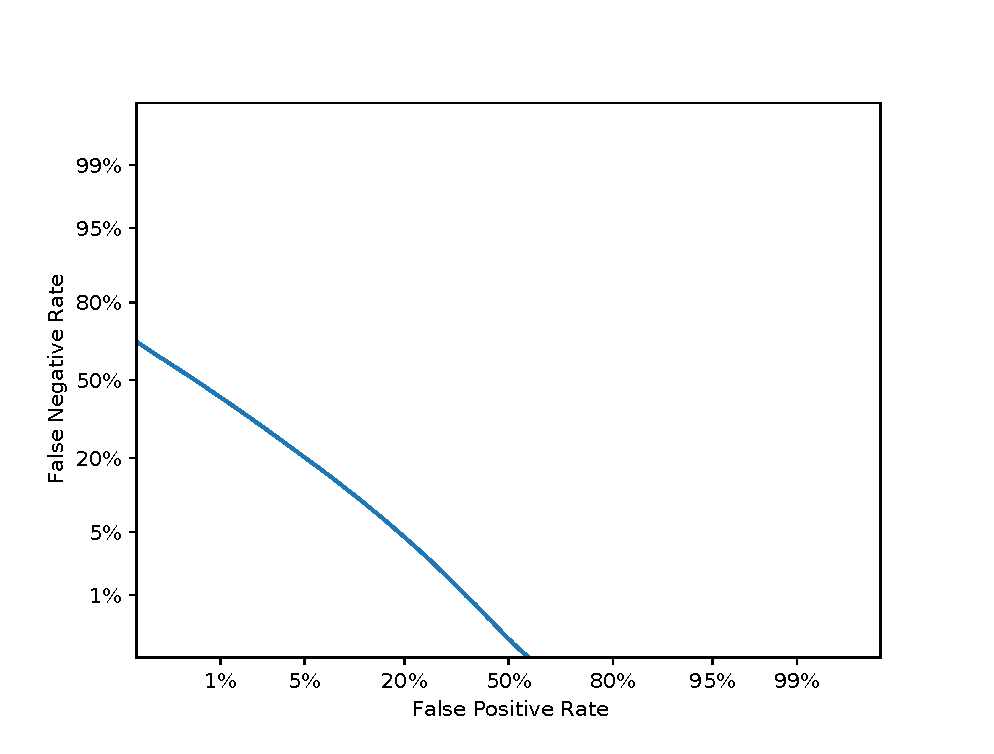
\includegraphics{det/softmax-relu.eps}}
		\caption{Softmax with ReLU}
	\end{subfigure}
	\begin{subfigure}[t]{7.5cm}
		\resizebox{7.5cm}{!}{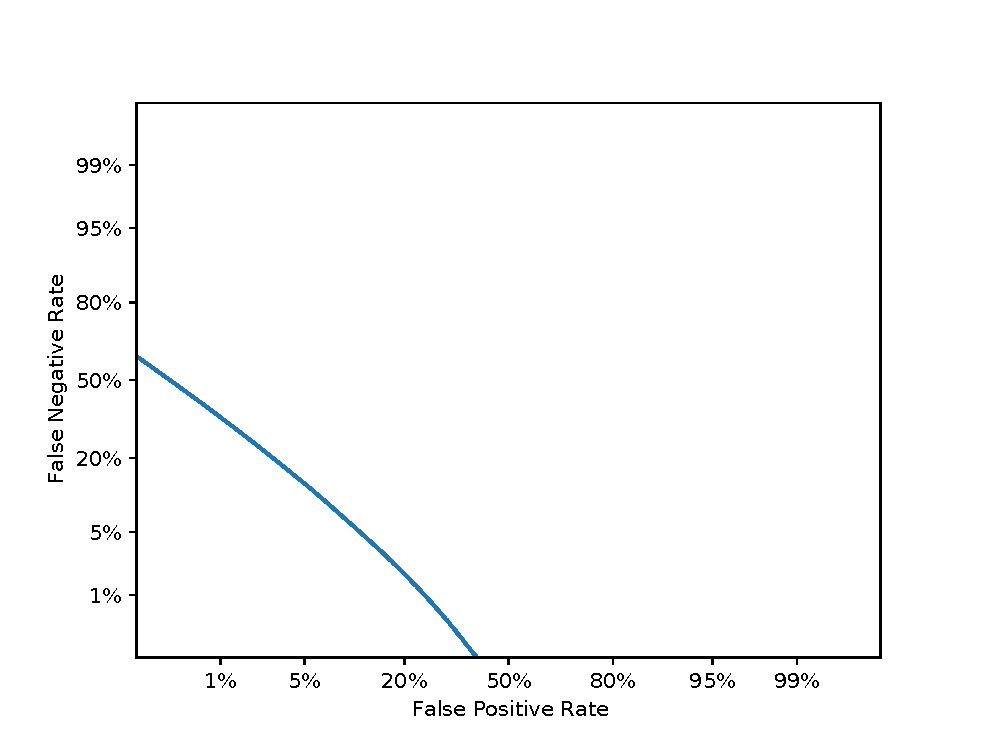
\includegraphics{det/A-softmax.eps}}
		\caption{Angular Softmax}
	\end{subfigure}
	\begin{subfigure}[t]{7.5cm}
		\resizebox{7.5cm}{!}{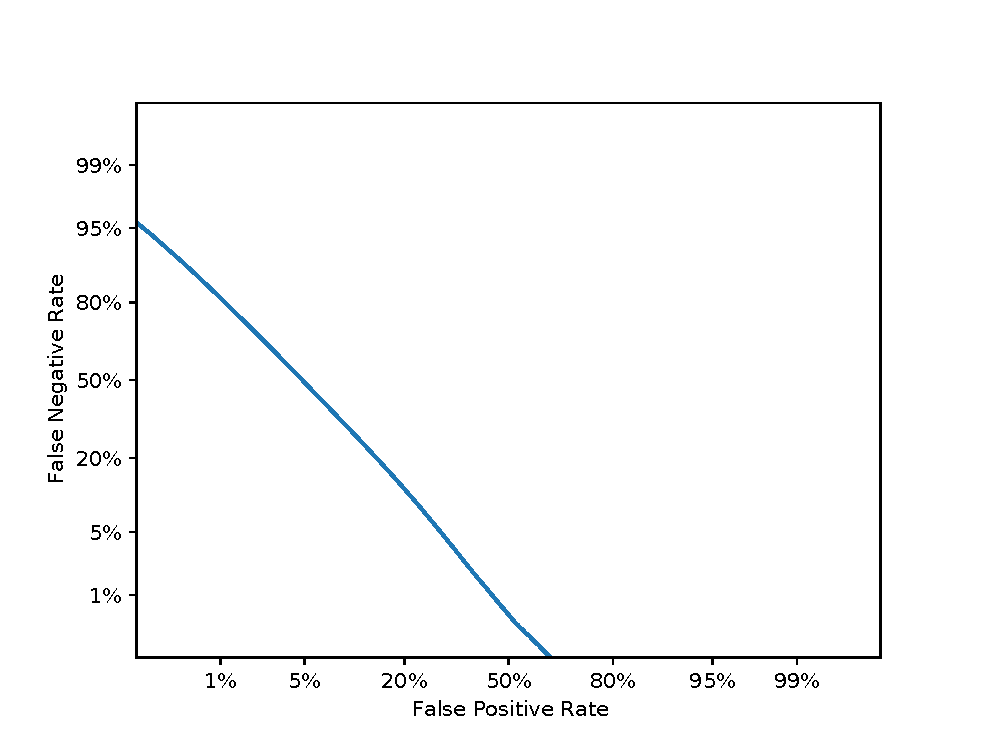
\includegraphics{det/triplet.eps}}
		\caption{Triplet margin L2}
	\end{subfigure}
\end{center}
\caption{DET curves}
\label{fig:det}
\end{figure}
